% ---------
%  Compile with "pdflatex hw0".  
% --------
%!TEX TS-program = pdflatex

\documentclass[letterpaper,11pt]{article}
\usepackage{jeffe,handout,graphicx}
\usepackage{fancyhdr}
\usepackage{comment}
\graphicspath{{./Fig/}}

\bibliographystyle{unsrt}
% ---------
% Input file uses Unicode's UTF-8 encoding
% ---------
%!TEX encoding = UTF-8 Unicode
\usepackage[T1]{fontenc}
\usepackage[utf8]{inputenc}

% ---------
%  The next several lines (up to the line of =='s) change the default text
%  and math fonts and make a few other minor cosmetic changes.  If you get
%  any error messages related to these packages, just comment them out.
%         -- Jeff
% --------
\usepackage[charter]{mathdesign}
 \def\sfdefault{fvs}
 \def\ttdefault{fvm}
 \SetMathAlphabet{\mathsf}{bold}{\encodingdefault}{\sfdefault}{b}{\updefault}
 \SetMathAlphabet{\mathtt}{bold}{\encodingdefault}{\ttdefault}{b}{\updefault}
 \SetMathAlphabet{\mathsf}{normal}{\encodingdefault}{\sfdefault}{\mddefault}{\updefault}
 \SetMathAlphabet{\mathtt}{normal}{\encodingdefault}{\ttdefault}{\mddefault}{\updefault}
 \usepackage{microtype}
% ---------
%  End of cosmetics.
% --------

\newcommand{\name}{Zigang Xiao (zxiao2), Yuelin Du (du6), Pei-Ci Wu (peiciwu1)} 
\newcommand{\hwnumber}{5}                % fill homework count
\newcounter{probid}
\newtheorem{definition}{Definition}
\newtheorem{theorem}{Theorem}
\newcommand{\hdr}[2]{
   \newpage\setcounter{page}{1}       % reset page counter
   \lhead{\fancyplain{}{\textbf{#1}}}
   \rhead{\fancyplain{}{\textbf{#2}}}
   \cfoot{\fancyplain{}{\thepage}}
}

\newcommand{\stmt}{
 \EMPH{I understand the course policies.}
}

\newcommand{\saystmt}{
($\bullet$) \EMPH{I understand the course policies.}
}

\newcommand{\newprob}{
\hdr{CS 573 HW\hwnumber}{\name{} HW\hwnumber{} \#\arabic{probid}}
\stepcounter{probid}
\item
}

% =========================================================
\begin{document}
\pagestyle{fancy}
\fancyhf{}
\small\sf	% typeset excetps from problems in a different, smaller font

\begin{enumerate}
% ---------------------------------------------------------
\newprob
\saystmt

Describe and analyze an algorithm to nest the boxes so that the number of
visible boxes is as small as possible.

\begin{solution}
  We assume one box can only contain \emph{exactly} one another box, i.e.,
  two boxes cannot be placed into the same box simultaneously.
  We reduce this problem to bipartite matching problem, and then 
  use Ford-Fulkerson algorithm to solve it.
  We construct a bipartite graph $G$ with vertex set $U \cup W$ as follows:
  \begin{itemize}
    \item Each box is a node in both $U$ and $W$.
    \item For a pair of node $u\in U$ and $v \in W$, if $u$ can be rotated so 
      that it can be contained in $v$, we add an edge $e=(u,v)$. 
  \end{itemize}

  Call two boxes are nested if one contains another.
  Let $N$ be the maximum number of nested boxes.
  Then, the number of visible boxes can be simply computed as $n-N$.

  \begin{theorem}
    The maximum number of nested boxes equals to $|M|$, where $|M|$ is the
    value of the size of the maximum matching in $G$.
  \end{theorem}

  \begin{proof}
    If we know the maximum number of nested boxes and how the boxes contain
    each other, we can transfer to a maximum matching in $G$ as follows: if $u$
    contains $v$, then we select $e=(u,v)$ in $G$, where $u\in U$ and $v\in W$.
    Since each box can contain exactly one another box, this is a valid
    matching.  Each time we place a box into another, the number of visible
    boxes is decreased by one.  Let $|M|$ be the final number of edges
    selected.  It is maximized according to the above procedure.  Otherwise,
    if there is a matching that has larger size, 
    there will be a better way to place the boxes.  
    This contradicts with the assumption.
    By contradiction, $M$ is a maximum matching.
    Moreover, the number of the nested boxes and the size of the maximum
    matching is $|M|$. 

    Conversely, if we know a maximum matching, we can find how to place the
    boxes into each other by placing $u$ into $v$ for each $e=(u,v)$ in $M$.
    Each $u \in U$ is matched exactly once, which means each box can be placed
    in another box only once. Thus this is a valid solution for the problem.
    Furthermore, this scheme must has the maximum number of nested boxes.
    Otherwise, if there is a better way to place the box, we can transform it
    to a matching that has a larger size. By contradiction, this is the best
    way to place the box.

    Finally, the size of the maximum matching is $|M|$, and equals to the
    number of nested boxes. 
  \end{proof}

  There are at most six permutation of width, height and depth. Hence for a
  pair of boxes, we can determine whether they can contain one another in
  constant time. Let there be $n$ boxes. Then, there are $2n$ nodes and at most
  $O(n^2)$ edges in $G$.  Hence, the maximum flow has value at most $O(n)$, and
  the Ford-Fulkerson algorithm runs in $O(n^3)$ time.

\end{solution}

% ---------------------------------------------------------
\newprob
\saystmt

Describe an efficient algorithm that either rounds $A$ in this fashion, or
reports correctly that no such rounding is possible.

\begin{solution}
  We can solve this problem by reducing it to maximum flows problem 
  with edge demands. The capacities and demands are all integers.
  Before we do that, 
  we first check that if the sum of each row (or column)
  is an integer. If not, we report that no such rounding is possible. 
  This is because after rounding, the sum of each row (or column) must be an
  integer.
  
  Now we assume the sum of each row (or column) is an integer.
  Let $R[1..m]$ be the sum of each row, and $C[1..n]$ be the sum of each
  column.  We construct a graph $G$ with vertex set $\{s,t\} \cup U \cup V$ as
  follows:
  \begin{itemize}
    \item Each row $i$ is a node $r_i$ in $U$.
    \item Each column $j$  is a node $c_i$ in $V$.
  \end{itemize}

  The edges consists of:
  \begin{itemize}
    \item an edge $e: s \rightarrow r_i$ with capacity $c(e)=d(e)=R[i]$
      for each $r_i \in U$.
    \item an edge $e: c_j \rightarrow t$ with capacity $c(e)=d(e)=C[j]$ 
      for each $c_j \in V$.
    \item an edge $e: r_i \rightarrow c_j $ with capacity 
      $c(e)=\lceil x_{ij} \rceil$ and demand $d(e) = \lfloor x_{ij} \rfloor$ 
      for each pair of $r_i \in U$ and $c_j \in V$.  
  \end{itemize} 

  \begin{theorem}
    The rounding exists if and only if there is a maximum flow that saturates
    every edge leaving from $s$. The rounding scheme consists of the flow
    values of edges $r_i \rightarrow c_j$.
  \end{theorem}
  \begin{proof}
    If we know a correct rounding scheme, we can transform it to a feasible
    maximum flow in $G$. For each $x_{ij}=A[i][j]$, we push the same amount of
    flow to edge $r_i \rightarrow c_j$. Since this rounding scheme is correct,
    the sum of rows and columns are correct, which means the flow conservation
    is satisfied and the edges leaving $s$ and the edges entering $t$ are all
    saturated.  Note that $\sum_i R[i] = \sum_j C[j]$.  Clearly, it is a
    feasible maximum flow.

    Conversely, if we have a maximum flow that saturates every edge leaving
    $s$, we can round each element $A[i][j]=f(e)$, where $e$ is the edge 
    $r_i \rightarrow  c_j$. The flow value $f(e)$ satisfies 
    wireless.illinois.edu$d(e)~\leq~f(e)~\leq~c(e)$. Moreover, the capacities and demands are all
    integer values, which means Ford-Fulkerson will compute an integer flow.
    Thus, each entry $x_{ij}=A[i][j]$ is rounded correctly to 
    $\lfloor x_{ij} \rfloor$ or $\lceil x_{ij} \rceil$.  Finally, the sum of
    rows and columns are the same as the corresponding capacity (or demand)
    values in edges $s\rightarrow r_i $ and $c_j \rightarrow t$.  Since all
    these edges are saturated, the sum of entries in any row or column are
    unchanged.  Thus, it is a valid rounding scheme.  \end{proof}

  Clearly, there are $O(m+n)$ vertices  and $O(mn)$ edges in $G$.
  Computing the sums and constructing the graph can be done in $O(mn)$ time.
  If we use Edmonds-Karp fat-pipe algorithm, we get an overall running time of 
  $O(VE^2)=O((m+n)\cdot m^2n^2)$.
\end{solution}

% ---------------------------------------------------------
\newprob
\saystmt

Describe and analyze an algorithm to compute a donation schedule, describing
how much money each voter should send to each candidate on each day, that
guarantees that every candidate gets enough money to win their election.  The
schedule must obey both Federal laws and individual voters' budget constraints.
If no such schedule exists, your algorithm should report that fact.

\begin{solution}
  Suppose there are $k$ days left from now to the election, there are $c$
  candidates and $v$ voters.  Let $M[1..c]$ be the money that must be spent on
  each candidate, $W[1..v][1..c]$ be the amounts that each voter is willing to
  donate to each candidate $A[1..v]$ be the total amounts that each voter is
  able to donate to all candidates.
  We can model this problem as a maximum flow problem.
  We construct a flow network $G=(V,E)$ with vertices $X \cup Y \cup \{s,t\}$,
  where each node in $X$ and $Y$ denotes a voter and a candidate, respectively.
  The edges consist of:
  \begin{itemize}
    \item an edge $s \rightarrow x$ with capacity $\min\{100, A[x]/k\}$ for
      each $x\in X$.
    \item an edge $y \rightarrow t$ with capacity $M[y]/k$ for each $y \in Y$.
    \item an edge $x \rightarrow y$ with capacity $W[x][y]/k$ for each $x\in X$
      and $y \in Y$.
  \end{itemize}

  \begin{theorem}
    The donation schedule exists if and only if there is a maximum flow that 
    saturates every edge entering $t$. The money that each voter should spend
    to each candidate on every day is denoted by the edges $x \rightarrow y$
    for each $x\in X$ and $y \in Y$.
  \end{theorem}

  \begin{proof}
    Given a maximum flow computed in $G$, we can convert it to a donation
    schedule as follows.  For each edges $x \rightarrow y$, it denotes the
    amount that voter $x$ will send to candidate $y$ each day.  For each edge
    $y \rightarrow t$ for each $y \in Y$, it denotes the amount that every
    candidate must receive each day to meet the campaign requirement.  For each
    edge $s \rightarrow x$ for each $x \in X$, clearly it satisfies both
    Federal lasw and individual voters' budget constraints.  If the maximum
    flow saturates all the edges entering $t$, then following this schedule,
    after $k$ days each candidate can receive exactly $M[y]$ money for all $y
    \in Y$.  Hence, the maximum flow we compute can be converted to a correct
    schedule.

    Conversely, if we have a correct donation schedule, we can convert it to a
    maximum flow in $G$ by pushing the same amount of flow as $W[x][y]/k$ on
    edge $x \rightarrow y$ for each $x\in X$ and $y\in Y$.  The donation
    schedule is correct, hence it satisfies the constraint on edges
    $s\rightarrow x$ for each $x \in X$.  Hence this is a feasible flow.
    Furthermore, the schedule can meet each candidate's requirement and thus
    all the edges entering $t$ will be saturated. Hence it is a maximum flow.
  \end{proof}

  The maximum flow has value at most $S=\sum_y M[y]$. There at most 
  $v + v \cdot c + c = O(vc)$ edges. Thus, Ford-Fulkerson algorithm
  runs in $O(Svc)$ time.
\end{solution}

% ---------------------------------------------------------
\newprob

\begin{enumerate}
  \item[($\bullet$)] \stmt
  \item 
Prove that this greedy strategy does not always compute an optimal solution.

\begin{solution}
  We prove by giving a counterexample. As in the following figure, 
  the blue cells are marked. Both of the 2-bend and 3-bend paths contains 
  maximum number of marked cells. However, if we choose the 2-bend path 
  at the first iteration, we need another two monotone path to cover all the
  cells. On the other hand, choosing the 3-bend path at first can finish 
  marking the cells with only two paths.
  \begin{center}
    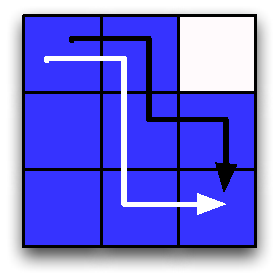
\includegraphics[width=.1\textheight]{p4}
  \end{center}
\end{solution}

\item
Describe and analyze an efficient algorithm to compute the smallest set of
monotone paths that covers every marked cell. The input to your algorithm is an
array $M[1..n,1..n]$ of booleans, where $M[i, j]$ = True if and only if cell
$(i, j)$ is marked.

\begin{solution}
  We can solve this problem by reducing it to a minimum-cost flow problem with
  demands.
  We construct a network $G$ as follows:
  \begin{itemize}
    \item For each cell $(i,j)$, we create two vertices $u_{i,j}$ and $v_{i,j}$.
      There is an edge $e: u_{i,j} \rightarrow v_{i,j}$ with cost 0.  If
      $M[i,j]=\mathsc{True}$, then $d(e)=1$. Otherwise $d(e)=0$.
      $u_{1,1}$ is the source vertex. $v_{n,n}$ is the target vertex.
    \item For each $v_{i,j}$, there are edges from $v_{i,j}$ to $u_{i+1,j}$ if
      $i+1 \leq n$, and $u_{i,j+1}$ if $j+1 \leq n$. 
      All of these edges have demands 0.
      For edges $v_{1,1} \rightarrow u_{2,1}$ and $v_{1,1} \rightarrow u_{1,2}$,
      they have cost 1. The rest has cost 0.
  \end{itemize}
  Let the number of smallest set of monotone paths that covers every marked cell
  be $k$.
  \begin{theorem}
    $k$ equals to the cost of the minimum-cost feasible flow in $G$.
    The set of monotone paths are the corresponding directed paths in $G$.
  \end{theorem}
  \begin{proof}
    If we know the smallest set of monotone paths, we can convert it 
    to a feasible flow in $G$ with cost $k$ by following the corresponding
    edges in $G$ according to the paths.
    Since every marked cell is visited, the edges with demand 1 
    are satisfied and thus the flow is feasible.
    The cost must be minimum. Otherwise, if there is a feasible flow with 
    smaller cost, we can convert it to a set of monotone paths that has 
    smaller size.
    
    Conversely, if we know a minimum-cost feasible flow with cost $k$, we 
    can convert it to a set of monotone paths.
    Since this flow is feasible, the demands are all satisfied, which 
    means the marked cells are all visited.
    $k$ is minimized. Otherwise, if there is a better way to construct 
    the set of paths, we can convert it back to find a feasible flow
    that has smaller cost.
  \end{proof}

  There are $O(n^2)$ vertices and edges in $G$. $G$ can be constructed 
  in $O(n^2)$ time.
  By running Sleator and Tarjan's network flow algorithm,
  our algorithm runs in $O(VE\log V)=O(n^4 \log n)$ time.
\end{solution}

\end{enumerate}


% ---------------------------------------------------------
\newprob

\begin{enumerate}
  \item[($\bullet$)] \stmt
  \item 
    Prove that if Paul uses a deterministic strategy, and Sally knows his
    strategy, then Sally can guarantee that she wins.
    \begin{solution}
      Since $r$ is a positive integer, $|S|>0$. If Sally knows 
      Paul's strategy, then she knows what path Paul will choose given 
      $s$ and $t$. She can simply choose the edge $e=(s,u)$ in this path and 
      win.
    \end{solution}

  \item 
    Describe a deterministic strategy for Sally that guarantees that she wins
    when $r \leq M$, no matter what strategy Paul uses.
    \begin{solution}
      Sally can just include all the $M$ edges that across the ($s$,$t$)-cut in
      $S$.  Imagine the path that Paul chooses as a flow from $s$ to $t$.
      Then, it must go through one of the $M$ edge in the minimum cut.  Since
      $S$ includes all these edges, $P \cap S$ must not be empty.
    \end{solution}

  \item 
    Prove that if Sally uses a deterministic strategy, and Paul knows her
    strategy then Paul can guarantee that he wins when $r < M$.
    \begin{solution}
      Let $M'$ be the number of edges in an arbitrary ($s$,$t$)-cut.
      It follows $M \leq M'$, and thus $r < M'$.
      Thus, Sally cannot choose all the edges that $P$ can possibly go through.
      Conversely, assume that there is no way for Paul to gurantee he wins. 
      It implies that all the edges in one of the minimum cut are included in
      $S$, and thus $r \geq M$. This contradicts with the $r < M$.  
      By contradiction, Paul can gurantee he wins.  
    \end{solution}

  \item 
    Describe a randomized strategy for Sally that guarantees that she wins with
    probability at least $\min\{r/M,1\}$, no matter what strategy Paul uses.
    \begin{solution}
      Suppose each edge is chosen independently and uniformly. The randomized
strategy for Sally is to randomly choose a subset $S$ of $r$ edges in the
minimum ($s, t$)-cut. Note if $r \ge M$, Sally chooses $M$ edges in the minimum
cut, i.e. all edges in the minimum cut are chosen by Sally.
\begin{itemize}
\item If $r \ge M$, $S$ contains all edges in the minimum cut. According to
  (b), the probability that Sally wins is 1.
\item If $r < M$, Sally has to choose at least one edge in $P$ to win. $P$ must
  contain at least one edge in the minimum cut. We first consider only one edge
  in the minimum cut is contained in $P$. Besides choosing the edge contained
  in $P$, Sally have to choose $r-1$ edges in other $M-1$ edges, so  the
  probability is
\[
\frac{\left(^{M-1}_{r-1}\right)}{\left(^M_r\right)} = \frac{r}{M}
\] 
Since $P$ contains at least one edge in the minimum cut, the probability that
the edges that Sally chooses are contained in $P$ is at least $r/M$. So when $r
< M$, the probability that Sally wins is at least $r/M$.
\end{itemize}
Thus, based on the two items above, the probability that Sally wins is at least
$\min$\{$r/M$, 1\}.

    \end{solution}
  \item 
    Describe a randomized strategy for Paul that guarantees that he loses with
    probability at most $\min\{r/M,1\}$, no matter what strategy Sally uses.
    \begin{solution}
Suppose each edge is chosen independently and uniformly. The randomized
strategy for Paul is to first randomly select an edge $e$ in the 
minimum ($s, t$)-cut, and then choose a path which passes $e$ among the maximum
flow. 

The largest probability that Paul loses is when Sally uses her best strategy to
win. In the following, we will compute the probability that Sally uses her best
strategy to win. 

\begin{itemize}
\item If $r \ge M$, the largest probability that Paul loses is 1 since no
  matter which edge $e$ Paul selects, Sally can choose all edges in the minimum
  cut. So the probability that Paul loses is at most 1.
\item If $r < M$, the edge $e$ has to be chosen by Sally so that Paul loses.
  The probability that edge $e$ is chosen when Sally chooses $r$ edges in the
  minimum cut is $r/M$ (according to the results of (d)). We can partition
  edges in $G$ into a set of cuts such that each cut has at most one edge in
  $P$. If an edge can be partitioned into more
  than one cuts, just partition it into any one of the cuts. Suppose $G$ can be
  partitioned into $n$ cuts, where the number of edges in the $n$ cuts is
  $M_1$, $M_2$, $\dots$, $M_n$, respectively. Let $r_1, r_2, \dots, r_n$ be the
  number of edges that Sally chooses in the $n$ respective cuts. So the
  possibility that Sally chooses at least one edges of $P$ in $G$ is
\begin{align*}
\textrm{Pr[Sally wins]} &\le \frac{r_1}{M_1} + \frac{r_2}{M_2} + \dots +
\frac{r_n}{M_n}
~~~~~~&(\mbox{since $M_1, M_2, \dots, M_n \le M$}) \\
&\le \frac{r_1 + r_2 + \dots + r_n}{M} 
~~~~~~&(\mbox{since $r_1 + r_2 + \cdots + r_n = r$}) \\
&= \frac{r}{M}
\end{align*}

Since $r/M$ is the probability that Sally wins by using her best strategy,
$r/M$ is the largest probability that Paul loses. So the probability that Paul
loses is at most $r/M$.
\end{itemize}
Thus, based on the two items above, the probability that Paul loses is at most
$\min$\{$r/M$, 1\}.

    \end{solution}

\end{enumerate}

% =========================================================

\end{enumerate}
\end{document}
